\chapter{Analysis}

\section[Reelle Zahlen]{Reelle Zahlen $\boldsymbol{\mathbb{R}}$}

\subsection{Angeordnete Körper}
\index{Angeordnete Körper}

(Gilt auch für $\mathbb{Z}$ und $\mathbb{Q}$)

\paragraph{Körperaxiome $\mathbf{(\mathbb{R}, +, *)}$}
\index{Körperaxiome}
$a,b,c \in \mathbb{R}$

\begin{description}
  \item [Addition $(\mathbb{R},+)$]
        \index{Addition}\
        \begin{description}
          \item [Assoziativität]
                \index{Assoziativität}
                $\linebreak a + (b + c) = (a + b) + c$

          \item [Kommutativität]
                \index{Kommutativität}
                $\linebreak a + b = b + a$

          \item [Neutrales Element Null]
                \index{Null}
                $\linebreak a + 0 = a \quad 0 \in \mathbb{R}$

          \item [Inverses ,,Negativ``]
                \index{Negatives}
                $\linebreak a + (-a) = 0 \quad (-a) \in \mathbb{R}$
        \end{description}

  \item [Multiplikation $(\mathbb{R},*)$]\
        \index{Multiplikation}
        \begin{description}
          \item [Assoziativität]
                \index{Assoziativität}
                $a * (b * c) = (a * b) * c$

          \item [Kommutativität]
                \index{Kommutativität}
                $a * b = b * a$

          \item [Neutrales Element Eins]
                \index{Eins}
                $\linebreak a * 1 = a \quad 1 \in \mathbb{R} \setminus \{ 0 \}$

          \item [Inverses ,,Kehrwert``]
                \index{Kehrwert}
                $\linebreak a * (a^{-1}) = 1$ \\
                $a \boldsymbol{\neq} \mathbf{0}, (a^{-1}) \in \mathbb{R}$
        \end{description}
  \item [Distributivität]
        \index{Distributivität}
        $\linebreak \mathbf{a} * (b + c) = \mathbf{a} * b + \mathbf{a} * c$
\end{description}

\paragraph{Totale Ordnung}

\begin{description}
  \item [Transitivität]
        \index{Transitivität der Ordnung}
        $\linebreak a < b \land b < c \Rightarrow a < c$

  \item [Trichotomie] Entweder \\
        \index{Trichotomie}
        \index{Irreflexivität der Ordnung}
        $a < b$ oder $a = b$ oder $b < a$ \\
        $\Rightarrow$ \emph{Irreflexivität} ($a < b \Rightarrow a \neq b$)

  \item [Addition]
        $\linebreak a < b \Rightarrow a + c < b + c$

  \item [Multiplikation]
        $\linebreak a < b \Rightarrow a * c < b * c \quad 0 < c$
\end{description}

% % Korrelat
% \paragraph{Notation}
% 
% \begin{align*}
%   a > b    & :\Leftrightarrow b < a            \\
%   a \leq b & :\Leftrightarrow a < b \lor a = b \\
%   a \geq b & :\Leftrightarrow a > b \lor a = b
% \end{align*}
% 
% \paragraph{Lemma}
% 
% \begin{itemize}
%   \item $a \leq a$
%   \item $a < b \Rightarrow a \neq b$
%   \item $a \leq b \lor b \leq a$
%   \item $a \leq b \land b \leq a \Rightarrow a = b$
%   \item $a < b \Rightarrow a * c \boldsymbol{>} b * c \quad 0 < c$
%   \item $a < b \land c < d \Rightarrow a + c < b + d$
%   \item $c < 0 \Leftrightarrow - c > 0$
%   \item $a \neq 0 \Rightarrow a^2 > 0$
%   \item $a < 0 \Rightarrow a^{-1} < 0$
%   \item $0 < a < b \Rightarrow b^{-1} < a^{-1}$
% \end{itemize}

Bei Additiver oder Multiplikativer Inversion dreht sich die Ungleichung.

\subsection{\textsc{Archimedes} Axiom}
\index{\textsc{Archimedes} Axiom}

\begin{align*}
  \forall x \in \mathbb{R} \exists n \in \mathbb{N}: & n > x           \\
                                                     & n > \frac{1}{x}
\end{align*}

\subsection{Teilbarkeit}
\index{Teilbarkeit}

$$a | b \Leftrightarrow \exists n \in \mathbb{Z}: b = a * n$$

($\Rightarrow \sqrt{2} \notin \mathbb{Q}$, da mit $\frac{a}{b} = \sqrt{2}$ nicht teilerfremd)
\index{Irrationalität}

\subsection{Häufige Fehler}

\begin{itemize}
  \item Nicht durch Null teilen/kürzen

  \item Nicht $-x < 0$ annehmen

  \item Multiplikation mit negativen Zahlen kehrt Ungleichungen
\end{itemize}

\subsection{Operationen}

\paragraph{Brüche}
\index{Bruch}

\begin{itemize}
  \item $\frac{a}{b} * \frac{c}{d} = \frac{a c}{b d}$

  \item $\frac{a}{b} \overset{\mathbf{* d}}{=} \frac{a \mathbf{d}}{b \mathbf{d}}$

  \item $\frac{a}{\mathbf{c}} + \frac{b}{\mathbf{c}} = \frac{a + b}{\mathbf{c}}$

  \item $\frac{a}{b} + \frac{c}{d} = \frac{ad + cb}{bd}$
\end{itemize}

\paragraph{Wurzeln} $b^n = a \Leftrightarrow b = \sqrt[n]{a}$
\index{Wurzel}

\begin{mzImportant}
  \begin{itemize}
    \item $\sqrt[n]{\mathbf{a * b}} = \sqrt[n]{\mathbf{a}} \mathbin{\boldsymbol{*}} \sqrt[n]{\mathbf{b}}$

    \item $\sqrt[\mathbf{n}]{ \sqrt[\mathbf{m}]{a} } = \sqrt[\mathbf{n * m}]{a}$

    \item $\sqrt[n]{a} < \sqrt[n]{b} \quad 0 \leq a < b$

    \item $\sqrt[n+1]{a} < \sqrt[n]{a} \quad 1 < a$

    \item $\sqrt[n]{a} < \sqrt[n+1]{b} \quad 0 < a < 1$
  \end{itemize}

  $$\sqrt[n]{a^n} = |a| \quad a \in \mathbb{R}$$
\end{mzImportant}


\paragraph{Potenzen} $a^{\frac{x}{y}} = \sqrt[y]{a^x}$
\index{Potenz}

\begin{mzImportant}
  \begin{itemize}
    \item $a^{\mathbf{x}} * b^{\mathbf{x}} = (a \mathbf{*} b)^{\mathbf{x}}$

    \item $a^x * a^y = a^{x \boldsymbol{+} y}$

    \item $(a^x)^y = a^{x \boldsymbol{*} y}$

          % \item $a^x < a^y \quad 1 < a, x < y$
          % \item $a^x > a^y \quad 0 < a < 1, x < y$
          % \item $a^x < b^x \quad a < b, 0 < x$
          % \item $a^x > b^x \quad a < b, x < 0$
  \end{itemize}
\end{mzImportant}


\subsection{Dezimaldarstellung}
\index{Dezimaldarstellung}

\paragraph{\textsc{Gauss}-Klammer}
\index{\textsc{Gauss}-Klammer}
$[y] := \max \{ k \in \mathbb{Z} \mid k \leq y \} = \floor{y}$

$$[y] = k \Leftrightarrow k \leq y < k + 1$$

\paragraph{Existenz} $\forall x \geq 0 \exists ! (a_n)_{n \in \mathbb{N}}$ mit

\begin{itemize}
  \item $a_n \in \{ 0, \dots, 9 \} \quad \forall n \in \mathbb{N}$
  \item $\sum_{i = 0}^n \frac{a_i}{10^i} \leq x < \sum_{i = 0}^n \frac{a_i}{10^i} + \frac{1}{10^n} \quad \forall n \in \mathbb{N}_0$
\end{itemize}

Die Umkehrung gilt mit Lemma:

\begin{mzImportant}
  $$x = \sum_{n = 0}^\infty \frac{a_n}{10^n}$$
\end{mzImportant}

\paragraph{Lemma} $x \geq 0$, $(a_n)_{n \in \mathbb{N}}$ Dezi. von $x$

$$\boldsymbol{\neg} (\exists N \in \mathbb{N} \forall n \geq N: a_n = 9)$$

$$x \in \mathbb{Q} \Leftrightarrow (a_n)_{n \in \mathbb{N}} \text{ periodisch}$$

\section{Intervalle}
\index{Intervall}

Sei $A \subseteq \mathbb{R}, A \neq \emptyset, a_0 \boldsymbol{\in} A$.

\begin{description}
  \item [Geschlossen]
        \index{Abgeschlossen}
        $[a;b] := \{ x \in \mathbb{R} \mid a \boldsymbol{\leq} x \boldsymbol{\leq} b \}$ \\
        (,,Ecken sind mit enthalten``)

  \item [Offen]
        \index{Offen}
        $(a;b) := \{x \in \mathbb{R} \mid a \boldsymbol{<} x \boldsymbol{<} b\}$ \\
        (Bei $\infty$ immer offen, da $\infty \notin \mathbb{R}$)
\end{description}

\paragraph{Kleinstes/Grö\ss tes Element}

\begin{mzImportant}
  \begin{description}
    \item [Minimum]
          \index{Minimum in $\mathbb{R}$}
          $\min(A) := a_0$ \\
          $\Leftrightarrow \forall a \in A: \mathbf{a_0} \boldsymbol{\leq} a$

    \item [Maximum]
          \index{Maximum in $\mathbb{R}$}
          $\max(A) := a_0$ \\
          $\Leftrightarrow \forall a \in A: \mathbf{a} \boldsymbol{\leq} a_0$
  \end{description}
\end{mzImportant}

($\nexists {}^{\min}/_{\max} (a;b)$)

\paragraph{Beschränktheit} $A$ hei\ss t
\index{Beschränkte Menge}

\begin{description}
  \item [Oben beschränkt]
        \index{Obere Schranken in $\mathbb{R}$}
        $\exists s \in \mathbb{R} \forall a \in A: \mathbf{a} \boldsymbol{\leq} s$

  \item [Unten beschränkt]
        \index{Untere Schranken in $\mathbb{R}$}
        $\exists s \in \mathbb{R} \forall a \in A: \mathbf{s} \boldsymbol{\leq} a$
\end{description}

\paragraph{Vollständigkeit}
\index{Vollständigkeit}

\begin{mzImportant}
  \begin{description}
    \item [Infimum (klein)] $\inf(A)$ \\
          \index{Reelles Infimum}
          $:= \mathbf{\max} \{ s \in \mathbb{R} \mid \forall a \in A: \mathbf{s} \boldsymbol{\leq} a \}$

    \item [Supremum (gro\ss)] $\sup(A)$ \\
          \index{Reelles Supremum}
          $:= \mathbf{\min} \{ s \in \mathbb{R} \mid \forall a \in A: \mathbf{a} \boldsymbol{\leq} s \}$
  \end{description}
\end{mzImportant}

\paragraph{Vollständigkeitsaxiom} $\exists \sup(A)$.
\index{Vollständigkeitsaxiom}

\mzGraphic{
  \begin{tikzpicture}
    \draw[->] (-3,0) -- (4,0);

    \draw
    (0,0) node[above=1.5] (interval) {$A$}

    (0,0) + (-1,0) node (links) {$[$}
    (0,0) + (1,0) node (rechts) {$]$}

    (links.north) node[above right] {$\min$}
    (links.west) node[below left] {$\inf$}

    (links.west) + (-1,0) node[above left] {\shortstack{Untere\\Schranken}}

    (rechts.north) node[above left] {$\max$}
    (rechts.east) node[below right] {$\sup$}

    (rechts.east) + (1,0) node[above right] {\shortstack{Obere\\Schranken}}

    (4,0) node[below right] {$\mathbb{R}$};

    \draw[color=primary,decorate,decoration=coil]
    (links) -- (rechts);
  \end{tikzpicture}
}

\section{Folgen}

\paragraph{Folge $\mathbf{(a_n)_{n \in \mathbb{N}}}$} in $A$ ist eine Abb. $f: \mathbb{N} \rightarrow A$ mit $a_n = f(n)$.
\index{Folge}

\begin{description}
  \item [Arithmetische Folge]
        \index{Arithmetische Folge}
        $a_{n+1} = a_n + d$ \\
        $a_n = a + (n-1) * d \quad d, a \in \mathbb{R}$

  \item [Geometrische Folge]
        \index{Geometrische Folge}
        $a_{n+1} = a_n * q$ \\
        $a_n = q^n \quad q \in \mathbb{R}$
\end{description}

\paragraph{Rekursion} $a_n$ ist auf $\mathbf{a_{n-1}}$ definiert.
\index{Rekursion}

\begin{align*}
  a_{n+1} = & F(n, a_n) \quad \forall n \in \mathbb{N} \\
            & F: A \times \mathbb{N} \rightarrow A
\end{align*}

\paragraph{Primfaktorzerlegung} $n\in \mathbb{N}, n \geq 2$
\index{Primfaktorzerlegung}

$$\exists p_1, \dots, p_n \in \mathbb{P}: n = \mathbf{p_1 * \cdots * p_n}$$

\subsection{Summen und Produkte}

\begin{description}
  \item [Summe] $\sum_{i = 1}^n i = 1 + 2 + \cdots + n$
        \index{Summ}

  \item [Produkt] $\prod_{i = 1}^n i = 1 * 2 * 3 * \cdots * n$
        \index{Produkt}

  \item [Fakultät] $n! = \prod^n i$ ($\mathbf{0! = 1}$)
        \index{Fakultät}
\end{description}

\paragraph{\textsc{Gaussche} Summe} $n \in \mathbb{N}$
\index{\textsc{Gaussche} Summenformel}

\begin{mzImportant}
  $$\sum^n i = \frac{n * (n + 1)}{2}$$
\end{mzImportant}

\begin{mzImportant}

  \paragraph{Geom. Summe} $q \in \mathbb{R} \setminus \{ 0 \}, n \in \mathbb{N}_0$
  \index{Geometrische Summe}

  $$\sum_{i=0}^n q^i = \frac{1 - q^{n+1}}{1 - q}$$

  \paragraph{\textsc{Bernoulli} Unglei.} $n \in \mathbb{N}_0, x \geq -1$
  \index{\textsc{Bernoulli} Ungleichung}

  $$(1 + x)^n \geq 1 + nx$$

  \paragraph{Binom. Koeff.} $\binom{n}{k} = \frac{n!}{k! (n - k)!}$
  \index{Binomial Koeffizient}
\end{mzImportant}

\begin{itemize}
  \item Rechnen: $\frac{n > k}{0 < (n - k)}$

  \item $\binom{n}{0} = \binom{n}{n} = 1$

  \item $\binom{n + 1}{k + 1} = \binom{n}{k} + \binom{n}{k + 1}$
\end{itemize}

\paragraph{Binomischer Satz} $n \in \mathbb{N}$
\index{Binomischer Satz}

\begin{mzImportant}
  $$(a + b)^n = \sum_{k=0}^n \binom{n}{k} * a^{n - k} b^k$$
\end{mzImportant}

\section{Grenzwerte}

\paragraph{Betrag} $|x| := \begin{cases}
      & x \quad 0 \leq x \\
    - & x \quad x < 0    \\
  \end{cases}$
\index{Betrag}

\begin{mzImportant}
  \begin{description}
    \item [Lemma] $|x * y| = |x| * |y|$

    \item [Dreiecksungleichung]
          \index{Dreiecksungleichung}
          $|x + y| \boldsymbol{\leq} |x| + |y|$

    \item [Umgekehrte \linebreak Dreiecksungleichung]
          \index{Umgekehrte Dreiecksungleichung}
          $\linebreak ||x| - |y|| \leq |x - y|$
  \end{description}
\end{mzImportant}

\subsection{Konvergenz}
\index{Konvergenz}

Sei $(a_n)_{n \in \mathbb{N}} \subseteq \mathbb{R}, a \in \mathbb{R}$.

\begin{mzImportant}
  \begin{gather*}
    a_n \xrightarrow{n \rightarrow \infty} a \Leftrightarrow \\
    \forall \epsilon > 0 \exists n_0 \in \mathbb{N} \forall n \in \mathbb{N} n \geq n_0: \\
    \mathbf{|a_n - a| \leq \epsilon} \\
    (a - \epsilon \leq a_n \leq a + \epsilon)
  \end{gather*}
\end{mzImportant}

\mzScale{0.5}{
  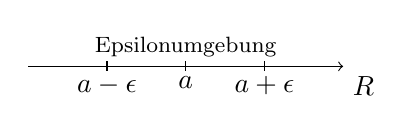
\begin{tikzpicture}
    \draw[->] (-2,0) -- (2,0) node[below right] {$\mathbb{R}$};

    \node at (0,0) (a) [below] {$a$};
    \node at (-1,0) (minus) [below] {$a - \epsilon$};
    \node at (1,0) (plus) [below] {$a + \epsilon$};

    \node at (a.north) [above] {\footnotesize Epsilonumgebung \index{Epsilonumgebung}};

    \draw (a.north) + (0,1/16) -- +(0,-1/16)
    (minus.north) + (0,1/16) -- +(0,-1/16)
    (plus.north) + (0,1/16) -- +(0,-1/16);
  \end{tikzpicture}
}

\begin{itemize}
  \item $a_n \xrightarrow{n \rightarrow \infty} a \Leftrightarrow \boldsymbol{\lim}_{n \rightarrow \infty} a_n = a$
        \index{Limes}
\end{itemize}

\begin{mzImportant}
  Beschränkt + monoton $\Rightarrow$ konvergent:

  $$\lim_{n \rightarrow \infty} a_n = \begin{cases}
      \boldsymbol{\inf} \{ a_n \mid n \in \mathbb{N} \} \quad (a_n)_\text{\emph{fall.}} \\
      \boldsymbol{\sup} \{ a_n \mid n \in \mathbb{N} \} \quad (a_n)_\text{\emph{steig.}}
    \end{cases}$$
\end{mzImportant}

\begin{description}
  \item [Nullfolgen] $\lim_{n \rightarrow \infty} a_n = \mathbf{0}$
        \index{Nullfolge}
        \begin{itemize}
          \item  $\lim_{n \rightarrow \infty} \frac{1}{n^k} = \mathbf{0} \quad k \in \mathbb{N}$

          \item $\lim_{n \rightarrow \infty} nq^n = \mathbf{0}$
        \end{itemize}

        \item[Folgen gegen $\mathbf{1}$]\
        % \index{Folge gegen Eins}

        \begin{itemize}
          \item $\lim_{n \rightarrow \infty} \sqrt[n]{a} = \mathbf{1} \quad a > 0$

          \item $\lim_{n \rightarrow \infty} \sqrt[n]{n} = \mathbf{1}$
        \end{itemize}

\end{description}

\paragraph{Bestimmt Divergent}
\index{Bestimmt Divergent}

\begin{mzImportant}
  \begin{gather*}
    a_n \xrightarrow{n \rightarrow \infty} \boldsymbol{\infty} \Leftrightarrow \\ \forall R \boldsymbol{>} 0 \exists n \geq n_0 \in \mathbb{N}: a_n \boldsymbol{\geq} R \\
    a_n \xrightarrow{n \rightarrow \infty} \boldsymbol{-\infty} \Leftrightarrow \\ \forall R \boldsymbol{<} 0 \exists n \geq n_0 \in \mathbb{N}: a_n \boldsymbol{\leq} R
  \end{gather*}
\end{mzImportant}

$$
  \lim_{n \rightarrow \infty} q^n \begin{cases}
    = \mathbf{0} \quad         & (-1; 1) \\
    = \mathbf{1} \quad         & = 1     \\
    \geq \mathbf{\infty} \quad & > 1     \\
    \mathbf{\text{div.}} \quad & \leq -1
  \end{cases}
$$

\paragraph{Monotonie} % $(a_n)_{n \in \mathbb{N}} \subseteq \mathbb{R}$
\index{Monotonie}

\begin{description}
  \item [Monoton fallend]
        \index{Monton fallend}
        $\linebreak a_n \underset{\text{(streng)}}{\boldsymbol{\geq}} a_{n + 1} \quad \forall n \in \mathbb{N}$

  \item [Monoton steigend]
        \index{Monoton steigend}
        $\linebreak a_n \underset{\text{(streng)}}{\boldsymbol{\leq}} a_{n + 1} \quad \forall n \in \mathbb{N}$
\end{description}

\paragraph{Beschränktheit} % $(a_n)_{n \in \mathbb{N}} \subseteq \mathbb{R}$
\index{Beschränkte Folge}

$$\exists k > 0 \forall n \in \mathbb{N}: \mathbf{|a_n| \leq k}$$

\begin{mzImportant}
  \begin{itemize}
    \item Konvergent $\Rightarrow$ beschränkt

    \item Unbeschränkt $\Rightarrow$ divergent
  \end{itemize}
\end{mzImportant}

\section{Grenzwertsätze}
\index{Grenzwertsätze}

$$\lim_{n \rightarrow \infty} a_n = a, \lim_{n \rightarrow \infty} b_n = b$$

\begin{itemize}
  \item $a_n \xrightarrow{n \rightarrow \infty} a \land a_n \xrightarrow{n \rightarrow \infty} b \linebreak \Rightarrow a = b$ (Max. einen Grenzw.)

  \item $a = \mathbf{0} \land (b_n)_\text{\emph{beschr.}}$ \\
        $\Leftrightarrow \lim_{n \rightarrow \infty} a_n b_n = \mathbf{0}$

  \item $a_n \boldsymbol{\leq} b_n \Leftrightarrow a \boldsymbol{\leq} b \quad (\text{nicht} <)$

  \item
        $\lim_{n \rightarrow \infty} \begin{cases}
            a_n \boldsymbol{\pm} b_n = a \boldsymbol{\pm} b                                                   \\
            a_n \boldsymbol{\divideontimes} b_n = a \boldsymbol{\divideontimes} b                             \\
            a_n \boldsymbol{\divideontimes} c = a \boldsymbol{\divideontimes} c                               \\
            \mathbf{\sqrt[\color{black}k]{\color{black}a_n}} = \mathbf{\sqrt[\color{black}k]{\color{black}a}} \\
            \boldsymbol{|}a_n\boldsymbol{|} = \boldsymbol{|}a\boldsymbol{|}
          \end{cases}$
\end{itemize}

\paragraph{Einschachtelungssatz}
\index{Einschachtelungssatz}
\index{Sandwichtheorem}

\begin{mzImportant}
  \begin{gather*}
    \lim_{n \rightarrow \infty} a_n = \lim_{n \rightarrow \infty} b_n = a \\
    \forall n \geq N \in \mathbb{N}: \mathbf{a_n \leq c_n \leq b_n} \\
    (\exists) \lim_{n \rightarrow \infty} c_n = \mathbf{a}
  \end{gather*}
\end{mzImportant}

\subsection{Spezielle Folgen}

\index{Teilfolge}
\paragraph{Teilfolge} \emph{streng mnt.} Folge $(b_k)_{n \in \mathbb{N}}$ mit $(n_k)_{k \in \mathbb{N}}$, sodass $b_k = \mathbf{{a_n}_k} \quad \forall k \in \mathbb{N}$.

\begin{mzImportant}
  $$\lim_{n \rightarrow \infty} a_n = a \Rightarrow \lim_{n \rightarrow \infty} {a_n}_k = a$$

  (da $n_k$ mnt. steigend)

  $$\forall (a_n)_{n \in \mathbb{N}} \exists {({a_n}_k)_{k \in \mathbb{N}}}_\text{\emph{mnt.}}$$

  (nicht streng!)
\end{mzImportant}

\paragraph{Häufungspunkt} $h$ mit einer Teilfolge
\index{Häufungspunkt}

$$\lim_{n \rightarrow \infty} {a_n}_k = h$$

\begin{itemize}
  \item $\lim_{n \rightarrow \infty} a_n = a \Leftrightarrow \exists!: h = a$
\end{itemize}

\paragraph{\textsc{Bolzano-Weierstra\ss}}
\index{\textsc{Bolzano-Weierstra\ss}}

\begin{mzImportant}
  $${(a_n)_{n \in \mathbb{N}}}_{\text{\emph{beschr.}}} \Rightarrow \exists h_\text{\emph{Häuf.}}$$

  (Beschränkte Teilfolgen besitzen mind. einen Häufungspunkt)
\end{mzImportant}

\subsection{\textsc{Cauchy}-Folge}
\index{\textsc{Cauchy}-Folge}

\begin{mzImportant}
  \begin{gather*}
    \forall \epsilon > 0 \exists n_0 \in \mathbb{N} \forall n, m \geq n_0:\\
    |a_n - a_m| \leq \epsilon
  \end{gather*}
\end{mzImportant}

(Konv. ohne bekannten Grenzwert)

\paragraph{Vollständigkeit von $\boldsymbol{\mathbb{R}}$}
\index{Vollständigkeit der Reelen Zahlen}

$${(a_n)_{n \in \mathbb{N}}}_\text{\emph{\textsc{Cauchy}}} \Leftrightarrow \exists \lim_{n \rightarrow \infty} a_n$$

\begin{align*}
  (\exists \lim_{n \rightarrow \infty} a_n
   & \Rightarrow {(a_n)_{n \in \mathbb{N}}}_\text{\textsc{Cauchy}} \\
   & \Rightarrow {(a_n)_{n \in \mathbb{N}}}_\text{beschr.}         \\
   & \Rightarrow \exists h \quad \text{\tiny (BW)}                 \\
   & \Rightarrow \lim_{n \rightarrow \infty} a_n = h)
\end{align*}

\subsection{Stetigkeit}

\begin{description}
  \item [Berührungspunkt]
        \index{Berührungspunkt}
        $D \subseteq \mathbb{R}, a \in \mathbb{R}$

        \begin{gather*}
          a \text{ BP. von } D \\
          \Leftrightarrow \exists (x_n)_{n \in \mathbb{N}} \text{ in } D: x_n \xrightarrow{n \rightarrow \infty} a \\
          \Leftrightarrow \forall \delta > 0 \exists x \in D: |x - a| \leq \delta
        \end{gather*}

  \item [Grenzwert gegen Stelle]
        \index{Grenzwert gegen Stelle}\
        $f: D \rightarrow \mathbb{R}, y \in \mathbb{R}, a \text{ BP. von } D$

        \begin{gather*}
          \lim_{x \rightarrow a} f(x) = y \\
          \Leftrightarrow \forall (x_n)_{n \in \mathbb{N}} \text{ in } D: \\ x_n \xrightarrow{n \rightarrow \infty} a \Rightarrow f(x_n) \xrightarrow{n \rightarrow \infty} y \\
          \Leftrightarrow \forall \epsilon > 0 \exists \delta > 0 \forall x \in D: \\
          |x - a| \leq \delta \Rightarrow |f(x) - y| \leq \epsilon
        \end{gather*}

        (Grenzwertsätze gelten analog)

  \item [Stetig an Stelle] $f$ stetig bei $a$
        \index{Stetigkeit}

        \begin{gather*}
          \lim_{x \rightarrow a} f(x) = f(a) \\
          \Leftrightarrow \forall (x_n)_{n \in \mathbb{N}} \text{ in } D: \\ x_n \xrightarrow{n \rightarrow \infty} a \Rightarrow f(x_n) \xrightarrow{n \rightarrow \infty} f(a) \\
          \Leftrightarrow \forall \epsilon > 0 \exists \delta > 0 \forall x \in D: \\
          |x - a| \leq \delta \Rightarrow |f(x) - f(a)| \leq \epsilon
        \end{gather*}

        (U.A. stetig: Summen, Produkte, Quotienten, Verkettungen stetiger Fkt. und Polynome)

  \item [Einseitiger Grenzwert]
        \index{Einseitiger Grenzwert}
        $x_0 {}^{<}/_{>} a \in D$

        \begin{gather*}
          \lim_{x {}^{\nearrow}/_{\searrow} a} f(x) = y \\
          \Leftrightarrow \forall (x_n)_{n \in \mathbb{N}} \text{ in } D: \\ (x_n \xrightarrow{n \rightarrow a} a \land  \mathbf{\forall n: x_n {}^{<}/_{>} a}) \\ \Rightarrow f(x_n) \xrightarrow{n \rightarrow \infty} y \\
          \Leftrightarrow \lim_{x \rightarrow a} f(x) = y \land x_0 {}^{<}/_{>} a \in D
        \end{gather*}

  \item [Grenzwert gegen $\infty$]
        \index{Grenzwert gegen Unendlich}
        $D$ unbeschränkt

        \begin{gather*}
          \lim_{x \rightarrow \infty} f(x) = y \\
          \Leftrightarrow \forall (x_n)_{n \in \mathbb{N}} \text{ in } D: \\
          x_n \xrightarrow{n \rightarrow \infty} \infty \Rightarrow f(x_n) \xrightarrow{n \rightarrow \infty} y \\
          \Leftrightarrow \forall \epsilon > 0 \exists x_0 \in \mathbb{R} \forall x \in D: \\
          x \geq x_0 \Rightarrow |f(x) - y| \leq \epsilon
        \end{gather*}

  \item [Grenzwert $= \infty$]
        \index{Grenzwert gleich Unendlich}

        \begin{gather*}
          \lim_{x \rightarrow a} f(x) = \infty \\
          \Leftrightarrow \forall (x_n)_{n \in \mathbb{N}} \text{ in }: \\
          x_n \xrightarrow{n \rightarrow \infty} a \Rightarrow f(x_n) \xrightarrow{n \rightarrow \infty} \infty \\
          \Leftrightarrow \forall R > 0 \exists \delta > 0 \forall x \in D: \\
          |x - a| \leq \delta \Rightarrow f(x) \geq R
        \end{gather*}
\end{description}

\subsection{Eigenschaften stetiger Funktionen}

\begin{description}
  \item[Lemma] $f(a) > \eta \Rightarrow \forall x \exists \delta > 0 \in D \cap [a - \delta, a + \delta]: f(x) > \eta$
  \item[Zwischenwert]
    \index{Zwischenwertsatz}
    $[a; b] \subseteq \mathbb{R}$, $f: [a; b] \rightarrow \mathbb{R}$ stetig, $f(a) \neq f(b)$

    \begin{gather*}
      f(a) < c < f(b) \\
      \Rightarrow \exists \xi \in (a; b): f(\xi) = c
    \end{gather*}

  \item [Korollar] $f(a) * f(b) < 0 \Rightarrow \exists \xi \in (a; b): f(\xi) = 0$
        (versch. Vorzeichen)

  \item [Satz]
        \begin{gather*}
          f: [a; b] \rightarrow \mathbb{R} \text{ stetig} \\
          \Rightarrow f \text{ beschränkt} \\
          \Rightarrow \exists {}^{\min}/_{\max} \{ f(x) \mid x \in [a; b] \}
        \end{gather*}

  \item [Satz] Sei $I$ Intervall, $I, J \subseteq \mathbb{R}$, $f: I \rightarrow J$ stetig, strg. mnt ($\Rightarrow$ injektiv), surjektiv
        \begin{gather*}
          \Rightarrow J \text{ Intervall} \\
          \Rightarrow f \text{ bijektiv} \\
          \Rightarrow f^{-1}: J \rightarrow I \text{ stetig}
        \end{gather*}
\end{description}

\section{Reihen}

\begin{description}
  \item [Reihe $(s_n)_{n \in \mathbb{N}} = \sum_{k=1}^\infty a_k$]
        \index{Reihe}
        mit den Gliedern $(a_k)_{k \in \mathbb{N}}$.

  \item [$n$te Partialsumme]
        \index{Partialsumme}
        $s_n = \sum_{k=1}^{\mathbf{n}} a_k$

  \item [Grenzwert] ebenfalls $\sum_{k=1}^{\boldsymbol{\infty}} a_k$, falls $s_n$ konvergiert
\end{description}

\paragraph{Spezielle Reihen}

\begin{mzImportant}
  \begin{description}
    \item[Geom.]
      \index{Geometrische Reihe}
      $\sum_{k=0}^\infty q^k = \frac{1}{1- q} \quad q \in (-1;1)$

    \item [Harmon.]
          \index{Geometrische Reihe}
          $\sum_{k=1}^\infty \frac{1}{k}$ divergent

    \item [Allg. Harmon.]
          \index{Allgemeine Harmonische Reihe}
          $\sum_{k=1}^\infty \frac{1}{k^\alpha}$ konvergiert $\forall \mathbf{\alpha > 1}$
  \end{description}
\end{mzImportant}

\paragraph{Lemma}

\begin{itemize}
  \item $\sum_{k=1}^\infty a_k$, $\sum_{k=1}^\infty b_k$ konvergent
        \begin{itemize}
          \item $\sum_{k=1}^\infty \mathbf{a_k} + \sum_{k=1}^\infty \mathbf{b_k} = \sum_{k=1}^\infty (\mathbf{a_k + b_k})$
          \item $\mathbf{c *} \sum_{k=1}^\infty \mathbf{a_k} = \sum_{k=1}^\infty \mathbf{c * a_k}$
        \end{itemize}

  \item $\exists N \in \mathbb{N}: (\sum_{k=\boldsymbol{N}}^\infty a_k)_\text{konv.} \Rightarrow (\sum_{k=\boldsymbol{1}}^\infty a_k)_\text{konv.}$ (Es reicht spätere Glieder zu betrachten)

  \item $(\sum_{k=1}^\infty a_k)_\text{konv.} \linebreak \Rightarrow \forall N \in \mathbb{N}: (\sum_{k=N}^\infty a_k)_\text{konv.} \linebreak \Rightarrow \lim_{N \rightarrow \infty} \sum_{k=N}^\infty a_k = 0$
\end{itemize}

\subsection{Konvergenzkriterien}

\begin{mzImportant}
  \begin{description}
    \item [\textsc{Cauchy}]
          \index{\textsc{Cauchy}-Kriterium}
          \begin{align*}
            \Leftrightarrow & {(\sum_{k=1}^n a_k)_{n \in \mathbb{N}}} \text{\emph{\textsc{ Cauchy}}} \\
                            & (\sum_{k=1}^\infty a_k)_\text{konv.}                                   \\
            \Leftrightarrow & \forall \epsilon > 0 \exists n_0 \in \mathbb{N} \forall n > m > n_0 :  \\
                            & | \sum_{k=m + 1}^n a_k | \leq \epsilon
          \end{align*}

    \item [Notwendig]
          \begin{align*}
            (\sum_{n=1}^\infty a_n)_\text{konv.} \Rightarrow \lim_{n \rightarrow \infty} a_n = \boldsymbol{0} \\
            \lim_{n \rightarrow \infty} a_n \neq 0 \Rightarrow (\sum_{n=1}^\infty a_n)_\text{div.}
          \end{align*}

    \item [Beschränkt]
          $a_n \geq 0$ ($\Rightarrow$ \emph{mnt.}) $\forall n \in \mathbb{N}$
          $$(\sum_{n=1}^\infty a_n)_\text{\emph{beschr.}} \Leftrightarrow (\sum_{n=1}^\infty a_n)_\text{konv.}$$

    \item [Majorante]
          \index{Majorantenkriterium}
          $0 \leq \mathbf{a_n \leq b_k} \quad \forall n \in \mathbb{N}$\\
          % (Min. $\leq$ Major.)
          \index{Majorante}
          \index{Minorante}
          $$(\sum_{n=1}^\infty b_n)_\text{konv.} \Leftrightarrow (\sum_{n=1}^\infty a_n)_\text{konv.}$$

    \item [Quotient]
          \index{Quotientenkriterium}
          $a_n \geq 0 \quad \forall n \in \mathbb{N}$
          $$
            \lim_{n \rightarrow \infty} \frac{a_{n + 1}}{a_n} \begin{cases}
              \mathbf{< 1} \rightarrow (\sum_{n = 1}^\infty a_n)_\text{konv.} \\
              \mathbf{> 1} \rightarrow (\sum_{n = 1}^\infty a_n)_\text{div.}
            \end{cases}
          $$

    \item [Wurzel]
          \index{Wurzelkriterium}
          $a_n \geq 0 \quad \forall n \in \mathbb{N}$
          $$
            \lim_{n \rightarrow \infty} \sqrt[n]{a_n} \begin{cases}
              \mathbf{< 1} \rightarrow (\sum_{n = 1}^\infty a_n)_\text{konv.} \\
              \mathbf{> 1} \rightarrow (\sum_{n = 1}^\infty a_n)_\text{div.}
            \end{cases}
          $$

    \item [Absolut]
          \index{Absolute Konvergent}
          $$(\sum_{n=1}^\infty | a_n |)_\text{konv.} \Rightarrow (\sum_{n=1}^\infty a_n)_\text{konv.}$$

          $$| \sum_{n=1}^\infty a_n | \leq \sum_{n=1}^\infty | a_n |$$

          (Dreiecksungleichung)
          \index{Reihendreiecksungleichung}

    \item [Leibniz] $(a_n)_{n \in \mathbb{N}}$ mnt. Nullfolge
          \index{Leibniz-Kriterium}
          $$(\sum_{n=1}^\infty (-1)^n * a_n)_\text{konv.}$$

    \item [Grenzwert] $a_n, b_n \geq 0 \quad \forall n \in \mathbb{N}$
          \index{Grenzwertkriterium}
          \begin{gather*}
            \lim_{n \rightarrow \infty} \frac{a_n}{b_n} \mathbf{> 0} \Rightarrow \\
            (\sum_{n=1}^\infty a_n)_\text{konv.} \Leftrightarrow (\sum_{n=1}^\infty b_n)_\text{konv.}
          \end{gather*}
  \end{description}
\end{mzImportant}


\subsection{Exponentialfunktion}
\index{Exponentialfunktion}

\begin{mzImportant}
  $$\exp(x) := \sum_{n = 0}^\infty \frac{x^n}{x!} = e^x$$
\end{mzImportant}

\begin{itemize}
  \item $\exp(0) = 1$
  \item
        \index{Eulersche Zahl}
        $\exp(1) = e \approx 2,71828 \notin \mathbb{Q}$ \\
        $e = \lim_{n \rightarrow \infty} (1 + \frac{1}{n})^n$
\end{itemize}

\begin{mzImportant}
  $$\exp(x) * \exp(y) = \exp(x + y)$$
\end{mzImportant}

\paragraph{\textsc{Cauchy}-Produkt}
\index{\textsc{Cauchy}-Produkt}

\begin{mzImportant}
  $$(\sum_{n = 0}^\infty a_n)(\sum_{n = 0}^\infty b_n) = \sum_{n = 0}^\infty \sum_{k = 0}^n a_k b_{n - k}$$
\end{mzImportant}

\paragraph{Korollar}

\begin{itemize}
  \item $\exp (x) > 0$
  \item $\frac{1}{\exp (x)} = \exp (-x)$
  \item $x < y \Rightarrow \exp (x) < \exp (y)$
  \item $\exp(r * x) = (\exp (x))^r$
  \item $\exp(r) = e^r$
\end{itemize}

$$\exp_a (x) := \exp(x * \log a) = a^x$$

\begin{itemize}
  \item $a > 1 \Rightarrow$ strng. mnt. steigend
  \item $0 < a < 1 \Rightarrow$ strng. mnt. fallend
  \item $0 < a \neq 1 \Rightarrow \exp_a: \mathbb{R} \rightarrow \mathbb{R}^+$ bijektiv
\end{itemize}

\subsection{Logarithmen}
\index{Logarithmus}

$$\log = \exp^{-1}: \mathbb{R}^+ \rightarrow \mathbb{R}$$

\begin{itemize}
  \item $\log 1/x = - \log x$
  \item $\log x/y = \log x - \log y$
  \item $\log x^r = r * \log x$
\end{itemize}

$$\log (x * y) = \log x + \log y$$

$$\log_a x = \frac{\log x}{\log a} = \exp_a^{-1}$$

% TODO: TikZ Graph of Log and Exp.

\subsection{Trigonometrische Funktionen}
\index{Trigonometrische Funktion}

$$\sin x := \sum_{k = 0}^\infty \frac{(-1)^k x^{2k + 1}}{(2k + 1)!}$$
\index{Sinus}

$$\cos x := \sum_{k = 0}^\infty \frac{(-1)^k x^{2k}}{(2k)!}$$
\index{Kosinus}

(beide absolut konvergent, $0^0 := 1$)

\begin{itemize}
  \item $|{}^{\sin}/_{\cos} x| \leq 1$
  \item $\sin - x = - \sin x$
  \item $\cos - x = \cos x$
  \item $\sin (x + y) = \sin(x) \cos(y) + \cos(x) \sin (y)$
        \index{Additionstheoreme}
  \item $\cos (x + y) = \cos(x) \cos(y) - \sin(x) \sin (y)$
  \item $\sin 2x = 2 \sin (x) \cos (x)$
  \item $\cos 2x = \cos^2 x - \sin^2 x$
  \item $\sin^2 x + \cos^2 x = 1$
        \index{Trigonometrischer \textsc{Pythagoras}}
  \item $\sin x - \sin y = 2 \cos (\frac{x + y}{2}) \sin(\frac{x - y}{2})$
  \item $\cos x - \cos y = 2 \sin (\frac{x + y}{2}) \sin(\frac{y - x}{2})$
\end{itemize}

$$\pi: \cos \frac{\pi}{2} = 0$$

% TODO: TikZ Graph of Sin and Cos and important values.

\begin{itemize}
  \item ${}^{\sin}/_{\cos} (x + 2\pi) = {}^{\sin}/_{\cos} x$
  \item ${}^{\sin}/_{\cos} (x + \pi) = - {}^{\sin}/_{\cos} x$
  \item ${}^{\sin}/_{\cos} (x + \frac{\pi}{2}) = {}^{\cos}/_{\sin} x$
  \item $\sin x = 0 \quad \forall k \in \mathbb{Z}: x = k \pi$
  \item $\cos x = 0 \quad \forall k \in \mathbb{Z}: x = (2k + 1) *\frac{\pi}{2}$
\end{itemize}

$$\tan x := \frac{\sin x}{\cos x}$$
\index{Tangens}

\section{Differenzierbarkeit}

$D \subseteq \mathbb{R}$, $f: D \rightarrow \mathbb{R}$, $a \in D$ BP von $D \setminus \{a\}$

\paragraph{Differenzierbar}
\index{Ableitung}
\index{Differenzierbarkeit}
an der Stelle $a$, falls

\begin{align*}
    & \lim_{x \rightarrow a} \frac{f(x) - f(a)}{x - a} =: f'(x) \\
  = & \lim_{h \rightarrow 0} \frac{f(a + h) - f(a)}{h}
\end{align*}

\begin{itemize}
  \item Differenzierbar bei $a \Rightarrow$ stetig bei $a$
\end{itemize}

\begin{description}
  \item [Summenregel]
        \index{Summenregel}
        $(f + g)'(a) = f'(a) + g'(a)$

  \item [Faktorregel]
        \index{Faktorregel}
        $(c * f)'(a) = c * f'(a)$

  \item [Produktregel]
        \index{Produktregel}
        $(f * g)'(a) = f'(a) * g(a) + f(a) * g'(a)$

  \item [Reziprokregel]
        \index{Reziprokregel}
        $(1/f)'(a) = - \frac{g'(a)}{g^2(a)}$

  \item [Quotientenregel]
        \index{Quotientenregel}
        $(f/g)'(a) = \frac{f'(a) * g(a) - f(a) * g'(a)}{g^2(a)}$

  \item [Kettenregel]
        \index{Kettenregel}
        $(f \circ g)'(a) = f'(g(a)) * g'(a)$

  \item [Umkehrfunktion]
        \index{Ableitung der Umkehrfunktion}
        $(f^{-1})'(b) = 1 / f'(f^{-1}(b))$
\end{description}

\mzGraphic{
  \begin{tblr}{
    cells = {c},
    hline{1-2,7,9,12} = {-}{},
      }
    $f'$                   & $f$          & $F$                           \\
    $0$                    & $a$          & $ax + c$                      \\
    $1$                    & $x$          & $\frac{1}{2} x^2 + c$         \\
    $-1/x^2$               & $1/x$        & $\ln (x) + c$                 \\
    $\frac{1}{2 \sqrt{x}}$ & $\sqrt{x}$   & $\frac{2}{3} x\sqrt{x} + c$   \\
    $ax^a - 1$             & $x^a$        & $\frac{1}{a + 1} x^a + 1 + c$ \\
    $\cos x$               & $\sin x$     & $-\cos(x) + c$                \\
    $-\sin x$              & $\cos x$     & $\sin(x) + c$                 \\
    $e^x$                  & $e^x$        & $e^x$                         \\
    $a^x \ln a$            & $a^x$        &                               \\
    $\frac{1}{x \ln a}$    & $\log_a x$   &
  \end{tblr}
}

Sei $f,g: [a, b] \rightarrow \mathbb{R}$ diffbar und stetig:

\paragraph{Satz von \textsc{Rolle}}
\index{Satz von \textsc{Rolle}}

$$f(a) = f(b) \Rightarrow \exists \xi \in (a, b): f'(\xi) = 0$$
% TODO: TikZ Grafik

\paragraph{Mittelwertsatz}
\index{Mittelwertsatz}

$$\exists \xi \in (a, b): f'(\xi) = \frac{f(b) - f(a)}{b - a}$$
% TODO: TikZ Grafik
\begin{gather*}
  \exists \xi \in (a, b): \\
  f'(\xi)(g(b) - g(a)) = g'(\xi)(f(b) - f(a))
\end{gather*}
\index{(Erweiterter) Mittelwertsatz}

\paragraph{Monotonie}

\begin{itemize}
  \item $(\forall x \in D: f(x) \leq 0) \Rightarrow f$ mnt. fallend
  \item $(\forall x \in D: f(x) < 0) \Rightarrow f$ strng. mnt. fallend
  \item $f$ (nicht streng) mnt. fallend $\Rightarrow \forall x \in D: f'(x) \leq 0$
\end{itemize}

\paragraph{Höhere Ableitungen}
\index{Höhere Ableitung}

\begin{description}
  \item[$n$-mal ableitbar] $\exists f', f'', \dots, f^{(n)}$
  \item[Stetig ableitbar] Ableitung stetig
\end{description}

\subsection{Extrema}

\paragraph{Lokales Extrema}
\index{Lokales Extrema}
\index{Lokales Minimum}
\index{Lokales Maximum}

\begin{gather*}
  \exists \epsilon > 0 \forall x \in D \cap (x_0 - \epsilon, x_0 + \epsilon):\\
  f(x_0) {}^{\leq}/_{\geq} f(x)
\end{gather*}

Ist $D$ Intervall und $x_0$ innerer Punkt und lokales Extremum:

$$\Rightarrow f'(x_0) = 0$$

(Achtung: Umkehrung nicht notwendig!)

Sei zusätzlich $f'(x_0) = 0$ und $f$ $2$-mal ableitbar:

\begin{itemize}
  \item $f''(x_0) < 0 \Rightarrow x_0$ lokales Maximum
  \item $f''(x_0) > 0 \Rightarrow x_0$ lokales Minimum
\end{itemize}

\subsection{Taylor-Polynome}

Sei $I \subseteq \mathbb{R}$, $a \in I$, $f: I \rightarrow \mathbb{R}$ $n$-mal diff.-bar

$$T_{n,a}^f(x) = \sum_{k=0}^{n} \frac{f^{(k)}(n)}{k!} (x - a)^k$$

\paragraph{Restglied (Lagrange)} $f$ $n+1$-mal diff.-bar

\begin{gather*}
  R_n (x) = f(x) - T_{n, a}^f (x) \\
  \Rightarrow \exists \xi \in (x, a): \\
  R_n(x) = \frac{f^{(n + 1)} (\xi)}{(n + 1)!} (x - a)^{n + 1}
\end{gather*}

\section{Integralrechnung}

\paragraph{Unterteilung} $(x_i)_{i = 0}^n \in [a, b]$ mit $a = x_0 < x_i < x_n = b$ (nicht notwendigerweise äquidistant)

\paragraph{Treppenfunktion} $\varphi: [a, b] \rightarrow \mathbb{R}$ mit $\exists (x_i)_{i = 0}^n \in [a, b] \forall (x_{i-1}, x_i): \varphi(x) = \text{konst.} = c_i$

\paragraph{Integral der Treppenfunktion}

$$I(\varphi) = \sum_{i=1}^{n} c_i (x_i - x_{i - 1})$$

Sei $\varphi, \psi \in T[a, b]$, $c \in \mathbb{R}$
\begin{itemize}
  \item $\varphi + \psi \in T[a, b]$, $c\varphi \in T[a, b]$
  \item $I(\varphi + psi) = I(\varphi) + I(\psi)$, $I(c\varphi) = cI(\varphi)$
  \item $\varphi \leq \psi \Rightarrow I(\varphi) \leq I(\psi)$
\end{itemize}

\paragraph{Unter-/Oberintegral} $f: [a, b] \rightarrow \mathbb{R}$ beschränkt

\begin{description}
  \item[Unteri.] $U(f) = \sup\{ I(\varphi) \mid \varphi \in T[a, b] \land \varphi \leq f \}$
  \item[Oberi.] $O(f) = \inf\{ I(\psi) \mid \psi \in T[a, b] \land \psi \geq f \}$
\end{description}

\paragraph{\textsc{Riemann}-Integral} $f: [a, b] \rightarrow \mathbb{R}$ beschränkt

$$U(f) = O(f) = \int_a^b f$$

\paragraph{Gleichmä\ss ig Stetig} $D \subseteq \mathbb{R}$, $f: D \rightarrow \mathbb{R}$

\begin{gather*}
  \forall \epsilon > 0 \exists \delta > 0 \forall x, y \in D: \\
  |x - y| \leq \delta \Rightarrow |f(x) - f(y)| \leq \epsilon
\end{gather*}

\begin{itemize}
  \item $f$ glm. stetig $\Rightarrow f$ stetig
  \item $f: [a, b] \rightarrow \mathbb{R}$ stetig $\Rightarrow f$ stetig
\end{itemize}

\paragraph{\textsc{Riemann}'sche Summe} $f,g: [a, b] \rightarrow \mathbb{R}$ ($\Rightarrow$ glm.) stetig

\begin{gather*}
  s_n(f) = \frac{b - a}{n} \sum_{i = 1}^{n} f(a + i\frac{b - a}{n}) \\
  \lim_{n \rightarrow \infty} s_n (f) = \int_{a}^{b} f
\end{gather*}

\begin{itemize}
  \item $\int f + g = \int f + \int g$
  \item $\int cf = c \int f$
  \item $f \leq g \Rightarrow \int f \leq \int g$
  \item $|\int f| \leq \int |f|$
  \item $\int_{a}^{b} f = \int_{a}^{c} f + \int_{c}^{b} f \quad a < c < b$
\end{itemize}

\paragraph{Mittelwertsatz} $f: [a, b] \rightarrow \mathbb{R}$ stetig

\begin{align*}
  \exists c \in [a, b]: & f(c) = \frac{1}{b -a} \int_{a}^{b} f \\
  \text{bzw. }          & A = \int_{a}^{b} f = (b - a) f(c)
\end{align*}